\chapter{色表示、強子與禁閉}

\paragraph{簡短的開場插曲。}
回到群論之前，容我先做一次不太要臉的商業宣傳。\emph{《黑洞戰爭》}講述了我與 Stephen Hawking 之間一場漫長的爭論：黑洞是否會摧毀量子資訊。書中也記錄了理論物理學家特有的一些殘酷玩笑：不只有薛丁格的貓，還有 Susskind 的魚，以及牠們不幸掉進馬桶的遭遇。這項任務完成後，我們回到 Alice 和 Bob。Alice 仍然很苦惱，因為 Bob 還在逼她學群論。

\lectureoverview{對稱性藉由作用於態而具有物理意義。我們先從旋轉談起，介紹表示與生成元，再將這套建構方式用於色\(SU(3)\)。色表示可以組合成強子，而其動力學則說明了為何從未觀測到孤立的色。}

\section{群及其作用對象}

每次討論對稱性，都包含兩個概念。第一個是抽象群：一組具有乘法法則、單位元與逆元的運算。第二個是這些運算所作用的對象。兩者可以區分，但在物理學中無法分開。對稱性之所以重要，是因為它會變換物理態、場、座標或可觀測量。

\begin{classroomqa}
\audiencequestion{群既被描述為抽象的乘法表，也被描述為作用於物理對象的矩陣。這兩個部分可以分開嗎？
\lecturetimestamp{00:01:58}}
\lecturerresponse{它們是不同層次的描述，但彼此完全相關。旋轉作為一種抽象運算，在我們指定它要旋轉什麼之前就已存在。接著，物理學要探討的是，同一個運算如何作用於特定系統相關的態與物理量。矩陣提供這種具體的作用，同時保留抽象的乘法法則。}
\end{classroomqa}

空間旋轉是最清楚的例子。在古典力學中，同一個旋轉可以作用於粒子的座標、磁鐵的方向，或任何其他向量。在量子力學中，態屬於線性向量空間，因此旋轉由作用於該空間的線性算符表示。若\(g\)表示抽象群元素，而\(D(g)\)表示其矩陣代表，則一致性要求
\begin{equation}
D(g_1g_2)=D(g_1)D(g_2),
\qquad
D(e)=\boldsymbol 1.
\end{equation}
矩陣不必與抽象運算長得相同，但矩陣的乘法必須重現群的乘法。
\editorialnote{同態方程明確寫出源文以文字說明的群乘法與矩陣乘法之間的對應關係。}

矩陣的維度由態空間決定，而不單由抽象群決定。若只考慮單一電子的自旋，就有兩種彼此正交的可能態：自旋向上與自旋向下；因此，態是二分量列向量。旋轉於是由\(2\times2\)矩陣表示。對兩個自旋為二分之一的物體，基底包含四個態，
\begin{equation}
\ket{\uparrow\uparrow},\qquad
\ket{\uparrow\downarrow},\qquad
\ket{\downarrow\uparrow},\qquad
\ket{\downarrow\downarrow},
\end{equation}
因此，旋轉在組合空間上的作用是四維的。

熟悉的序列如下：
\begin{equation}
\begin{array}{c|c|c}
\text{spin} & \text{number of states} & \text{matrix dimension}\\
\hline
0 & 1 & 1\times1\\
\frac12 & 2 & 2\times2\\
1 & 3 & 3\times3\\
\frac32 & 4 & 4\times4
\end{array}
\end{equation}
依此類推。自旋為零的態構成平凡表示：任何旋轉都不改變它。一乘一矩陣就是\(1\)。自旋為一的態有三個分量，其旋轉矩陣就是熟悉的三維向量旋轉。一般而言，自旋\(j\)的表示有\(2j+1\)個態。

表示也可以是無限維的。若我們描述電子完整的軌道運動，而不只考慮它的自旋，態就包含每個位置的振幅，或等價地，包含每個動量的振幅。此時，旋轉算符作用於無限維的波函數空間。因此，同一個抽象旋轉群可以有平凡、二維、三維與無限維表示。從自旋轉而討論色時，我們會再次用到這個事實。

\section{為什麼自旋旋轉屬於特殊酉群}

現在回到單一電子的自旋，並略去其軌道運動。旋轉以一個\(2\times2\)酉矩陣\(U\)表示，
\begin{equation}
U^\dagger U=\boldsymbol 1,
\qquad
U^{-1}=U^\dagger.
\label{eq:l4-unitarity}
\end{equation}
逆變換必須還原原來的旋轉，而酉性會保留範數，因而保留所有機率。

一般的\(2\times2\)複矩陣含有四個複數元素，也就是八個實參數。方程式~\eqref{eq:l4-unitarity}施加四個獨立的實條件，剩下四個參數。普通的空間旋轉只有三個參數：兩個用來選擇旋轉軸，一個用來選擇旋轉角。因此，這個酉矩陣多了一個相位。還需要加上以下限制：
\begin{equation}
\det U=1.
\label{eq:l4-det-one}
\end{equation}
參數計數於是為
\begin{equation}
8-4-1=3.
\end{equation}

行列式為一的條件在矩陣乘法下保持不變，因為
\begin{equation}
\det(AB)=\det A\,\det B.
\end{equation}
若兩個矩陣的行列式皆為一，其乘積的行列式也為一。這個條件也與酉性相容。對方程式~\eqref{eq:l4-unitarity}兩邊取行列式，得到
\begin{equation}
1=\det(U^\dagger U)
=\det(U^\dagger)\det U
=(\det U)^*\det U.
\end{equation}
因此，酉矩陣的行列式位於單位圓上：
\begin{equation}
\det U=e^{i\phi}.
\end{equation}

\begin{classroomqa}
\audiencequestion{酉性是否要求行列式為實數？
\lecturetimestamp{00:12:10}}
\lecturerresponse{不要求。酉性只要求模長為一。行列式可以是任意純相位\(e^{i\phi}\)。對二維矩陣而言，將\(U\)乘上\(e^{-i\phi/2}\)，即可消去共同相位，得到行列式為一的矩陣。}
\end{classroomqa}

確實，若
\begin{equation}
V=e^{-i\phi/2}U,
\end{equation}
則\(V\)仍然是酉矩陣，而且
\begin{equation}
\det V=e^{-i\phi}\det U=1.
\end{equation}
行列式為一的酉矩陣構成\(SU(2)\)。

有一點需要留意。很容易把\(SU(2)\)說成就是三維空間的旋轉群，但兩者之間是二對一的對應。矩陣\(U\)與\(-U\)對旋量的作用不同，卻對應到普通向量的同一個旋轉。因此
\begin{equation}
SU(2)/\{\boldsymbol 1,-\boldsymbol 1\}\simeq SO(3).
\end{equation}
在目前的討論中，重要的是局部乘法結構與三個生成元；雙重覆蓋則說明了自旋為二分之一的粒子為何具有二值旋轉性質。

\section{無窮小變換與其生成元}

有限旋轉可以由許多極小旋轉組成。接近單位元的群元素稱為無窮小元素。在連通群中，只要知道所有無窮小方向，就足以透過反覆相乘重建有限變換。對物理學更重要的是，生成這些無窮小變換的算符，就是與對稱性相關的守恆量。

將接近單位元的元素寫成
\begin{equation}
U=\boldsymbol 1+i\epsilon T,
\qquad |\epsilon|\ll1.
\label{eq:l4-infinitesimal-u}
\end{equation}
因子\(i\)是為了方便而採用的慣例。將此式代入酉性條件，並略去\(\epsilon^2\)階的項，可得
\begin{align}
(\boldsymbol 1+i\epsilon T)
(\boldsymbol 1-i\epsilon T^\dagger)&=\boldsymbol 1,
\\
i\epsilon(T-T^\dagger)&=0,
\\
T&=T^\dagger.
\label{eq:l4-hermitian-generator}
\end{align}
生成元是厄米算符，正如量子力學中的可觀測量必須具備的性質。

\begin{figure}[htbp]
\centering
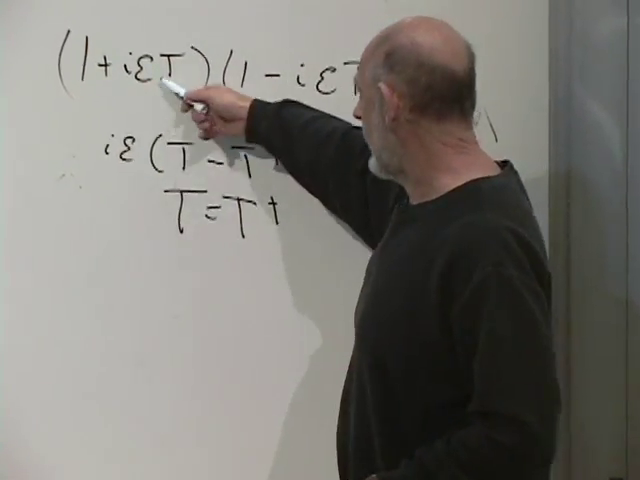
\includegraphics[width=0.62\textwidth]{lecture_04_figure_03.png}
\caption{接近單位元時的酉性計算，結果為\(T=T^\dagger\)。}
\lectureframe{00:23:28}
\end{figure}

空間旋轉有三個線性獨立的生成元，因為有三個獨立的無窮小旋轉軸。繞任意方向的微小旋轉，都可以由繞\(x\)、\(y\)和\(z\)的微小旋轉組成。相應的生成元是角動量算符\(J_x,J_y,J_z\)。它們的對易關係體現了旋轉的不對易性：
\begin{equation}
[J_i,J_j]=i\epsilon_{ijk}J_k.
\label{eq:l4-angular-momentum-algebra}
\end{equation}
反覆施行無窮小旋轉，便能構成有限旋轉。

我們已經使用酉性，但還沒有用到行列式為一的條件。對任意小矩陣\(m\)，
\begin{equation}
\det(\boldsymbol 1+\epsilon m)
=1+\epsilon\,\operatorname{tr}m+O(\epsilon^2).
\label{eq:l4-det-expansion}
\end{equation}

\begin{figure}[htbp]
\centering
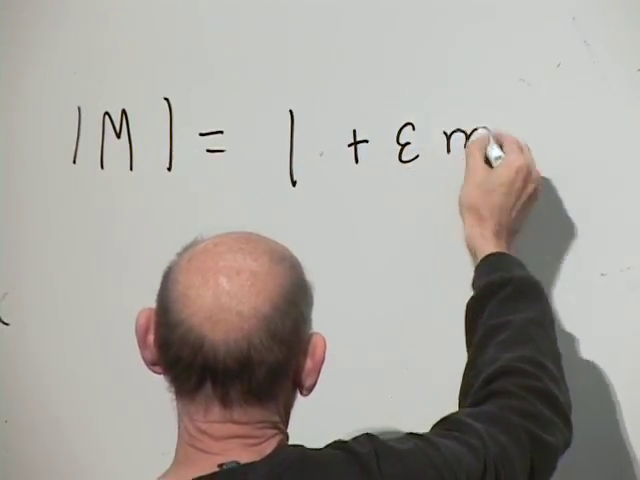
\includegraphics[width=0.62\textwidth]{lecture_04_figure_02.png}
\caption{黑板上推導行列式的一階展開。}
\lectureframe{00:21:51}
\end{figure}

將方程式~\eqref{eq:l4-det-expansion}應用於
方程式~\eqref{eq:l4-infinitesimal-u}，可得
\begin{equation}
\det U
=1+i\epsilon\,\operatorname{tr}T+O(\epsilon^2).
\end{equation}
因此，特殊酉條件要求
\begin{equation}
\operatorname{tr}T=0.
\label{eq:l4-traceless-generator}
\end{equation}
\(SU(2)\)的生成元正是無跡厄米\(2\times2\)矩陣。這個向量空間的維度為三。泡利矩陣構成一組標準基底：
\begin{equation}
\begin{aligned}
\sigma_x&=
\begin{pmatrix}0&1\\1&0\end{pmatrix},
&
\sigma_y&=
\begin{pmatrix}0&-i\\i&0\end{pmatrix},
\\[0.4em]
\sigma_z&=
\begin{pmatrix}1&0\\0&-1\end{pmatrix}.
\end{aligned}
\end{equation}
對自旋為二分之一的表示，可以取\(J_i=\sigma_i/2\)。因此，繞\(\hat{\boldsymbol n}\)旋轉角度\(\theta\)的有限旋轉為
\begin{equation}
U(\hat{\boldsymbol n},\theta)
=\exp\!\left(-i\theta\,
\hat{\boldsymbol n}\cdot\boldsymbol\sigma/2\right).
\end{equation}
\editorialnote{有限指數式是無窮小生成元討論的標準延伸。源文著重於反覆施行小旋轉，沒有明確寫出這個公式。}

\begin{classroomqa}
\audiencequestion{所以有三個線性獨立的無跡厄米\(2\times2\)矩陣？
\lecturetimestamp{00:24:07}}
\lecturerresponse{是的，就是三個泡利矩陣。對\(3\times3\)特殊酉矩陣，相應的數目是八；一組慣用基底是八個 Gell-Mann 矩陣。}
\end{classroomqa}

\begin{classroomqa}
\audiencequestion{這個「八」，和八重道以及八種膠子中的``八''是同一個意思嗎？
\lecturetimestamp{00:24:43}}
\lecturerresponse{數學上都涉及\(SU(3)\)表示論，但必須說清楚是哪一種\(SU(3)\)對稱性在作用。歷史上的八重道味對稱性不是色\(SU(3)\)。八種膠子則屬於色\(SU(3)\)的伴隨表示。}
\end{classroomqa}

\section{從 SU(2) 到色 SU(3)}

現在將矩陣從\(2\times2\)擴大到\(3\times3\)。一般的複數\(3\times3\)矩陣有九個複數元素，也就是十八個實參數。條件\(U^\dagger U=\boldsymbol 1\)提供九個實約束，而\(\det U=1\)再去掉一個參數。因此
\begin{equation}
18-9-1=8.
\end{equation}
有八個獨立的無窮小方向，以及八個無跡厄米生成元。與\(SU(2)\)不同，這個群不是普通三維空間的旋轉群，而是作用於色的內部對稱性。

在把這些表示指定給夸克之前，先回顧複合表示如何形成。將兩個自旋為二分之一的系統組合起來，並忽略它們的軌道運動。共有四個乘積態，但旋轉不會不可約地混合這四個態。其中三個組合按自旋一變換：
\begin{align}
\ket{1,1}&=\ket{\uparrow\uparrow},\\
\ket{1,0}&=\frac{1}{\sqrt2}
(\ket{\uparrow\downarrow}+\ket{\downarrow\uparrow}),\\
\ket{1,-1}&=\ket{\downarrow\downarrow},
\end{align}
第四個則按自旋零變換：
\begin{equation}
\ket{0,0}=\frac{1}{\sqrt2}
(\ket{\uparrow\downarrow}-\ket{\downarrow\uparrow}).
\end{equation}
因此
\begin{equation}
\boldsymbol 2\otimes\boldsymbol 2
=\boldsymbol 3\oplus\boldsymbol 1.
\label{eq:l4-two-spin-decomposition}
\end{equation}
對齊的態給出三重態中\(m=\pm1\)的成員；對稱的零投影態補足三重態，而反對稱組合則是單態。這就是角動量相加以及色表示組合的一般原理。

每當兩個自旋為二分之一的自由度耦合，都會出現同樣的單態--三重態區分。在氫原子中，電子與質子的自旋形成超精細單態和三重態。正氫與仲氫的兩個質子，其核自旋也遵循相同的表示論；這裡所指的是\(H_2\)分子。
\editorialnote{源文在提到氫原子中的質子--電子自旋時，使用了``正氫與仲氫''。數學上的分解是正確的；為求精確，此處區分了分子與原子的名稱。}

\subsection{三重態與反三重態}

單一夸克有三個色振幅。在選定的基底中，可寫成
\begin{equation}
q=
\begin{pmatrix}
q_r\\q_g\\q_b
\end{pmatrix},
\qquad
q'=Uq,
\qquad U\in SU(3).
\label{eq:l4-quark-triplet}
\end{equation}
這三個分量可以是單一夸克的態振幅，也可以是分別產生紅、綠、藍夸克的三個場算符。群會混合這三個分量。原本為紅色的態，經過色變換後，通常會成為紅、綠、藍的疊加態。這個基本的三維表示稱為\(\boldsymbol 3\)。

對反夸克而言，群透過夸克表示的複共軛表示作用。對方程式~\eqref{eq:l4-quark-triplet}取複共軛，得到
\begin{equation}
\bar q'=U^*\bar q.
\end{equation}
這個表示記作\(\bar{\boldsymbol 3}\)。與\(U(1)\)的類比很直接：若電子場獲得\(e^{i\theta}\)，正電子場便獲得\(e^{-i\theta}\)。夸克與反夸克的色變換，是這種共軛配對在非阿貝爾情形下的版本。

在單位元附近，若
\begin{equation}
U=\boldsymbol 1+i\epsilon T,
\end{equation}
則
\begin{equation}
U^*=\boldsymbol 1-i\epsilon T^*.
\end{equation}
因此，反三重態的生成元是\(-T^*\)，也就是帶有相反符號的共軛生成元。這就是反夸克帶有相反色荷的精確含義。

\begin{classroomqa}
\audiencequestion{在\(SU(2)\)的情況下，複共軛表示會如何？
\lecturetimestamp{00:36:19}}
\lecturerresponse{\(SU(2)\)二重態是特殊情況：經過一個涉及反對稱 epsilon 張量的固定基底變換後，其複共軛表示與原二重態等價。對\(SU(3)\)而言，\(\boldsymbol 3\)與\(\bar{\boldsymbol 3}\)則是真正不等價的表示。}
\end{classroomqa}
\editorialnote{\(SU(2)\)基本表示在數學上精確的術語是「偽實」，而非「實」。這段回答保留了源文要表達的區別，同時修正了術語。}

\section{色表示的組合}

符號\(\otimes\)並非表示將旁邊寫出的數字作普通乘法，而是表示組合兩個態空間。所得的張量積空間接著可重新分解為幾個部分；在群作用下，這些部分彼此不會混合。

\subsection{兩個夸克：\texorpdfstring{\(\boldsymbol 3\otimes\boldsymbol 3\)}{3 x 3}}

兩個夸克共有九個色基底態：紅--紅、紅--綠、紅--藍，以及其餘六種有序配對。將兩個色指標分成對稱部分與反對稱部分。對稱部分有六個獨立分量，反對稱部分有三個。在\(SU(3)\)下，
\begin{equation}
\boldsymbol 3\otimes\boldsymbol 3
=\boldsymbol 6\oplus\bar{\boldsymbol 3}.
\label{eq:l4-three-times-three}
\end{equation}

\begin{figure}[htbp]
\centering
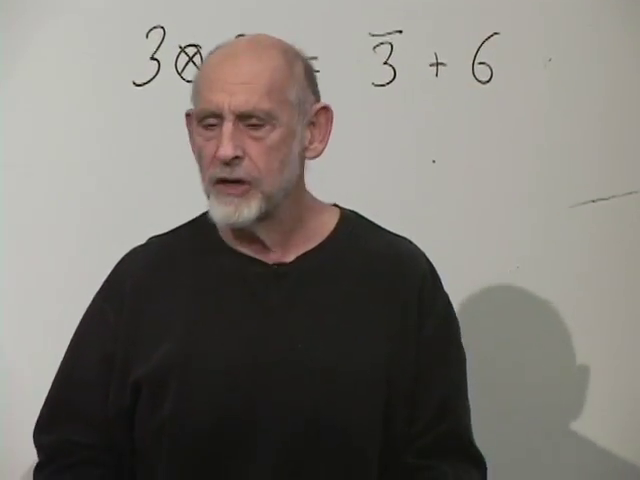
\includegraphics[width=0.68\textwidth]{lecture_04_figure_04.png}
\caption{兩個夸克的乘積分解為反三重態與六重態。}
\lectureframe{00:39:33}
\end{figure}

反三重態可以透過不變 epsilon 張量與兩個夸克指標縮併，明確表示為
\begin{equation}
(qq)^k_{\bar 3}
=\frac{1}{\sqrt2}\epsilon^{kij}q_iq_j.
\end{equation}
這個對象有三個分量，變換方式與反夸克相同。六種對稱組合構成六重態。這並不是說兩個夸克在動力學上變成反夸克，而是說其色波函數中的一個部分，具有與反夸克相同的變換律。

\subsection{一個夸克與一個反夸克：\texorpdfstring{\(\boldsymbol 3\otimes\bar{\boldsymbol 3}\)}{3 ⊗ 反3}}

夸克--反夸克色態可以視為一個\(3\times3\)矩陣\(M_i{}^j=q_i\bar q^j\)。每個這樣的矩陣都可以唯一分解為跡部分與無跡部分：
\begin{equation}
M=\frac{\operatorname{tr}M}{3}\boldsymbol 1
+\left(M-\frac{\operatorname{tr}M}{3}\boldsymbol 1\right).
\end{equation}
跡部分是單一的不變分量，無跡部分則有八個分量。因此
\begin{equation}
\boldsymbol 3\otimes\bar{\boldsymbol 3}
=\boldsymbol 1\oplus\boldsymbol 8.
\label{eq:l4-three-times-threebar}
\end{equation}
單態的形式如下，差一個歸一化因子：
\begin{equation}
\ket{1}_{q\bar q}
=\frac{1}{\sqrt3}
(\ket{r\bar r}+\ket{g\bar g}+\ket{b\bar b}).
\end{equation}
它是不變的，因此不會變換成其他態。其餘八個線性組合會彼此混合，構成伴隨表示；八個生成元也在同一表示中變換。

\subsection{三個夸克}

將第三個夸克與方程式~\eqref{eq:l4-three-times-three}所示的分支組合。反三重態分支給出
\begin{equation}
\bar{\boldsymbol 3}\otimes\boldsymbol 3
=\boldsymbol 1\oplus\boldsymbol 8,
\end{equation}
所以三夸克乘積包含一個單態。完整分解為
\begin{equation}
\boldsymbol 3\otimes\boldsymbol 3\otimes\boldsymbol 3
=\boldsymbol 1\oplus\boldsymbol 8\oplus\boldsymbol 8
\oplus\boldsymbol{10}.
\label{eq:l4-three-quark-full}
\end{equation}
色單態是完全反對稱的紅--綠--藍組合：
\begin{equation}
\ket{1}_{qqq}
=\frac{1}{\sqrt6}\epsilon^{ijk}\ket{q_iq_jq_k}.
\label{eq:l4-baryon-singlet}
\end{equation}
只要有兩個指標相同，\(\epsilon^{ijk}\)就會消失。因此，每個非零項都包含一個紅夸克、一個綠夸克和一個藍夸克；交換指標時，符號會交替。

\begin{classroomqa}
\audiencequestion{非單態組合只是出現機率很低，所以可以忽略它們的機率嗎？
\lecturetimestamp{00:46:02}}
\lecturerresponse{不可以。關鍵在於能量，而不是機率很小。孤立的非單態會使色場延伸至任意遠處；在禁閉區域中，這需要無界大的能量。下文會進一步說明這個說法背後的動力學。}
\end{classroomqa}

\subsection{膠子八重態}

膠子場的變換方式與方程式~\eqref{eq:l4-three-times-threebar}中的八重態相同。就色而言，它帶有一個三重態指標和一個反三重態指標，並扣除單態跡部分。概略地說，
\begin{equation}
q\sim\boldsymbol 3,
\qquad
\bar q\sim\bar{\boldsymbol 3},
\qquad
G\sim\boldsymbol 8.
\end{equation}
這些符號表示變換律；粒子並不等同於數字三或八。

第九種夸克--反夸克色組合與單位矩陣成正比，構成一個單態，不會與八重態混合。因此，省略這個單態在數學上是自洽的：\(SU(3)\)規範場是無跡的，含有八個分量；\(U(3)\)規範場則有九個分量。

\begin{classroomqa}
\audiencequestion{為什麼自然界省略了額外的單態膠子？
\lecturetimestamp{00:49:00}}
\lecturerresponse{直接的群論答案是：單態屬於獨立的不變子空間，因此即使不包含單態，八重態也能構成封閉的表示。此處不推導選擇\(SU(3)\)而非\(U(3)\)的更深層原因；這是從 QCD 現象學推知的規範結構之一。}
\end{classroomqa}

\section{色單態與強子}

強相互作用中自由且質量有限的粒子都是色單態。這不表示夸克或膠子並不存在，而是表示它們不會以孤立的漸近粒子形式出現。形成單態的基本模式如下：
\begin{equation}
qqq,
\qquad
q\bar q,
\qquad
GG\ \text{and higher gluonic products}.
\end{equation}
它們依序形成重子、介子與膠球。若干已無色的對象組合起來，當然仍然無色，因此還可以由這些成分構成更複雜的多強子態。

\begin{classroomqa}
\audiencequestion{三夸克單態與夸克--反夸克單態各稱為什麼？膠子也能組成單態嗎？
\lecturetimestamp{00:51:38}}
\lecturerresponse{三夸克單態稱為重子；夸克--反夸克單態稱為介子。膠子也可以組合成色單態。這類強相互作用態中最簡單的稱為膠球，參與組合的膠子也可以多於兩個。}
\end{classroomqa}

三個自旋為二分之一的夸克，總自旋必為半整數；不過，軌道角動量會影響最後得到哪個半整數。夸克--反夸克介子的自旋為整數。純膠子的膠球自旋也為整數。

對兩個膠子而言，黑板上的第一個陳述只是在計數：
\begin{equation}
8\times8=1+63.
\end{equation}
總共有六十四個色態，其中一個組合是單態，其餘六十三個屬於非單態子空間。

\begin{figure}[htbp]
\centering
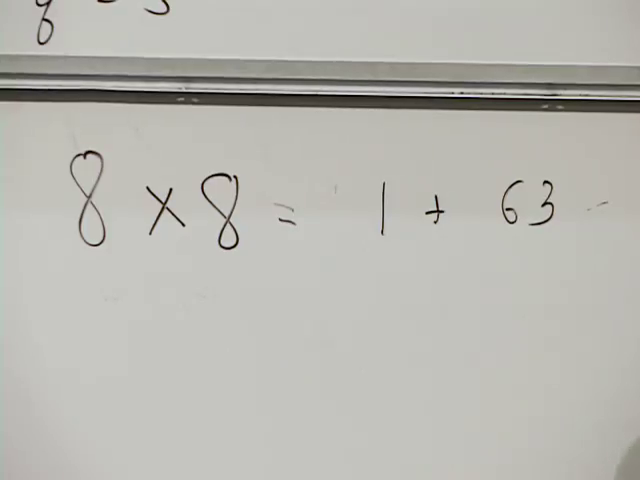
\includegraphics[width=0.68\textwidth]{lecture_04_figure_05.png}
\caption{黑板上的雙膠子態計數：六十四個態中有一個單態。}
\lectureframe{00:53:44}
\end{figure}

完整的不可約分解為
\begin{equation}
\boldsymbol 8\otimes\boldsymbol 8
=\boldsymbol 1\oplus\boldsymbol 8_S\oplus\boldsymbol 8_A
\oplus\boldsymbol{10}\oplus\overline{\boldsymbol{10}}
\oplus\boldsymbol{27}.
\label{eq:l4-eight-times-eight}
\end{equation}
維度相加無誤：
\begin{equation}
1+8+8+10+10+27=64.
\end{equation}
兩個八重態是不同的不變子空間；其中一個在交換兩個伴隨表示因子時對稱，另一個則反對稱。單態則是可以形成膠球態的雙膠子色道。
\editorialnote{黑板上最初只寫出\(8\times8=1+63\)。隨後的課堂問答提供了列出的不可約表示維度；此處依標準\(SU(3)\)記號補上橫線與對稱性標記。}

\subsection{為什麼可觀測到的電荷是整數}

夸克電荷分為兩種：
\begin{equation}
Q_{\mathrm{up\text{-}like}}=+\frac23,
\qquad
Q_{\mathrm{down\text{-}like}}=-\frac13.
\end{equation}
因此三個夸克的總電荷必為整數：\(-1,0,+1,\text{ or }+2\)，取決於其中有多少個是上型夸克。夸克與反夸克組成的態，電荷也會是\(0\)或\(\pm1\)。膠子不帶電。因此，由已觀測到的夸克表示所構成的基本色單態，電荷都是整數，儘管其中的組分帶有分數電荷。

\begin{classroomqa}
\audiencequestion{奇異夸克帶多少電荷？
\lecturetimestamp{00:56:08}}
\lecturerresponse{它屬於下型夸克，因此電荷為\(-1/3\)。三個世代都遵循相同的電荷模式：\((u,d)\)、\((c,s)\)與\((t,b)\)，每一對中的電荷分別是\(+2/3\)與\(-1/3\)。}
\end{classroomqa}

對這些粒子而言，色單態條件與整數電荷密切相關，但兩者並非相同的數學陳述。整數電荷也仰賴剛才列出的標準模型電荷配置。

\begin{classroomqa}
\audiencequestion{色單態是糾纏態嗎？它和貝爾實驗中的糾纏對具有相同的意義嗎？
\lecturetimestamp{00:56:58}}
\lecturerresponse{單態的色波函數確實是糾纏態：它是相干疊加，而不是各自具有確定顏色的乘積態。原則上，組分可以分離；但禁閉會使分離所需的能量愈來愈高，最後產生新的強子。因此，即使這個態確實糾纏，仍不適合用來進行貝爾實驗式的操控。}
\end{classroomqa}

\section{張量積方程式的意義}

現在值得更具體地說明這些乘法表。設\(\psi_i\)與\(\phi_j\)是用來產生兩個自旋為二分之一的物體的算符。它們可以描述兩種不同粒子，例如電子與質子；也可以描述同種粒子的兩個副本，但須納入適當的統計性質。每個指標有兩種取值。四個乘積
\begin{equation}
\psi_\uparrow\phi_\uparrow,
\quad
\psi_\uparrow\phi_\downarrow,
\quad
\psi_\downarrow\phi_\uparrow,
\quad
\psi_\downarrow\phi_\downarrow
\end{equation}
張成張量積空間。

若群元素在每個因子上的作用都是\(U\)，那麼它在乘積空間上的作用就是\(U\otimes U\)。用分量表示為
\begin{equation}
\psi_i\phi_j
\longmapsto
U_i{}^kU_j{}^\ell\psi_k\phi_\ell.
\label{eq:l4-product-action}
\end{equation}
這是四維表示，但它是可約的。反對稱組合
\begin{equation}
\frac{1}{\sqrt2}
(\psi_\uparrow\phi_\downarrow
-\psi_\downarrow\phi_\uparrow)
\end{equation}
在變換下仍映射至自身，而三個對稱組合則彼此映射。採用適合這些組合的基底後，每個乘積表示矩陣都會呈現區塊對角形式：
\begin{equation}
D_{2\otimes2}(g)
\sim
\begin{pmatrix}
1&0\\
0&D_3(g)
\end{pmatrix}.
\label{eq:l4-spin-block-diagonal}
\end{equation}

\begin{classroomqa}
\audiencequestion{像\(\boldsymbol 3\otimes\boldsymbol 3=\bar{\boldsymbol 3}\oplus\boldsymbol 6\)這樣的方程式表示什麼運算？
\lecturetimestamp{00:57:51}}
\lecturerresponse{左側表示組合後的態空間。群同時作用於兩個因子，因此會混合乘積基底中的各個態。右側表示經過基底變換後，這些態分成不變的子空間：三個反對稱組合按反三重態變換，六個對稱組合按六重態變換。加號表示不同子空間的直和，不是普通的數值相加。}
\end{classroomqa}

\begin{classroomqa}
\audiencequestion{我們怎麼知道九個態會分解成\(3+6\)或\(1+8\)，而不是例如\(2+7\)？
\lecturetimestamp{01:04:39}}
\lecturerresponse{光靠維度計數無法決定分解方式。必須知道\(SU(3)\)有哪些不可約表示，並建構不變子空間，例如將指標對稱化或反對稱化，或分離跡與無跡部分。完整分類需要更多群論；此處只使用討論夸克與膠子所需的表示。}
\end{classroomqa}

不變 epsilon 張量讓單態的構造一目了然。對於
\(SU(2)\)，
\begin{equation}
\epsilon_{ij}U^i{}_kU^j{}_\ell
=(\det U)\epsilon_{k\ell}
=\epsilon_{k\ell}.
\end{equation}
因此\(\epsilon_{ij}\psi^i\phi^j\)是不變的。對於\(SU(3)\)，三個指標的版本給出
\begin{equation}
\epsilon_{ijk}U^i{}_aU^j{}_bU^k{}_c
=(\det U)\epsilon_{abc}
=\epsilon_{abc},
\end{equation}
這便證明了方程式~\eqref{eq:l4-baryon-singlet}中的三夸克態是不變的。

\begin{classroomqa}
\audiencequestion{可以明確說明單態為何不會改變嗎？
\lecturetimestamp{01:07:18}}
\lecturerresponse{可以。用完全反對稱的 epsilon 張量縮併所有基本表示指標。經過變換後，矩陣的乘積會使 epsilon 張量乘上\(\det U\)。對特殊酉矩陣而言，這個行列式為一，因此縮併後的態保持不變。在\(SU(2)\)中，這證明了雙自旋單態的不變性；在\(SU(3)\)中，則證明紅--綠--藍三夸克單態的不變性。}
\end{classroomqa}

\begin{classroomqa}
\audiencequestion{兩個膠子八重態的完整分解是什麼？
\lecturetimestamp{01:09:24}}
\lecturerresponse{分解如方程式~\eqref{eq:l4-eight-times-eight}所示：一個單態、兩個八重態、一個十重態、一個反十重態，以及一個二十七維表示。兩個八重態指標恰好只有一種色單態組合。}
\end{classroomqa}

\begin{classroomqa}
\audiencequestion{三個夸克的完整分解又是什麼？
\lecturetimestamp{01:11:51}}
\lecturerresponse{物理上最重要的是，分解中包含一個單態。補完整個分解，就得到方程式~\eqref{eq:l4-three-quark-full}：一個單態、兩個八重態與一個十重態，總計\(1+8+8+10=27\)個態。\editorialnote{講者在問答中沒有想起完整的\(3\otimes3\otimes3\)分解。此處明確補上標準分解，並註明這是補充內容，而非講者口頭回答的一部分。}}
\end{classroomqa}

同樣的想法也可推廣到雙膠子空間。在樸素的乘積基底中，
\(SU(3)\)由\(64\times64\)矩陣表示。在適合不可約分量的基底中，這些矩陣呈區塊對角形式，
\begin{equation}
\begin{aligned}
D_{8\otimes8}(g)
&\sim
\operatorname{diag}\bigl(
1,D_{8_S}(g),D_{8_A}(g),
\\
&\hspace{4.8em}
D_{10}(g),D_{\overline{10}}(g),D_{27}(g)
\bigr).
\end{aligned}
\end{equation}
各區塊彼此不混合，但每個區塊內的態仍會相互混合。

\begin{classroomqa}
\audiencequestion{張量積分解是否只是換到某個基底，使大型表示矩陣呈現區塊對角形式？
\lecturetimestamp{01:12:02}}
\lecturerresponse{正是如此。兩個自旋的四維矩陣會分解成一個一維單態區塊和一個三維三重態區塊。兩個膠子的六十四維矩陣則會分解成維度為\(1,8,8,10,10,\text{ and }27\)的區塊。每個區塊在群的所有變換下都保持封閉。}
\end{classroomqa}

\begin{classroomqa}
\audiencequestion{完整張量積空間中，那些封閉部分之一有專門名稱嗎？
\lecturetimestamp{01:14:55}}
\lecturerresponse{它是不變子空間，承載著一個子表示。若它無法再分解，就承載著不可約表示，簡稱 irrep。完整的張量積是這些不可約分量的直和。\editorialnote{來源在課堂上沒有解答所詢問的術語；回答中補上了表示論的標準術語。}}
\end{classroomqa}

\begin{classroomqa}
\audiencequestion{把非單態十重態和其他表示稱為不存在，是否表示應該完全忽略它們？
\lecturetimestamp{01:15:36}}
\lecturerresponse{它們是合理的色扇區，在中間計算中也很重要，但不會在實驗室中以孤立的有限能量粒子形式出現。阻止它們成為自由漸近態的是禁閉，而不是表示論失效。}
\end{classroomqa}

\section{從南部的色荷構想談禁閉}

色荷的構想早於 QCD 的最終表述。早在1960年代初，南部陽一郎就已理解，一個隱藏的三值量子數可以解決一個引人注目的問題：夸克帶有分數電荷，但從未觀察到自由的分數電荷粒子。如果物理態必須是色單態，夸克就會以如上所述的整數電荷組合出現。剩下的是動力學問題：是什麼迫使所有有限能量的自由態都成為單態？

先從電磁類比談起。一個電荷與異號電荷相吸。將兩者拉近會降低能量；將同號電荷推近則需要做功。場本身儲存正能量，
\begin{equation}
E_{\mathrm{field}}
=\frac12\int d^3x\,\boldsymbol E^2
\end{equation}
以簡單的靜電單位表示。淨電荷會使電場延伸至系統之外很遠的地方，而緊密束縛的中性對只有短程的偶極場。因此，中和會移除系統外部的場能。

假設電磁耦合大幅增強。淨電荷所帶來的場能代價會變得極大，低能物體因而幾乎都會是中性的；抽離其中帶電的組分也可能變得代價高昂。南部將這種直覺應用於色荷：八種色荷是八種膠子場的源，因此巨大的色場能可能使孤立的非單態無法存在。

這種直覺基本上正確，但 QCD 有一項關鍵的新特徵。光子不帶電荷，膠子卻帶有色荷。光子不是經典電磁場的源，而且麥克斯威方程是線性的：兩個電磁波可以疊加並彼此穿過。膠子在色八重態表示中變換，因此膠子會成為其他膠子的源，並與其他膠子相互作用。甚至同一個膠子場的不同部分也會彼此作用。因此，非阿貝爾規範場是非線性的。

\subsection{通量管與線性勢}

在長距離下，膠子的自相互作用會阻止色通量像一般電偶極場那樣擴散。通量會被擠壓成一根連接夸克與反夸克的管。長通量管的場強和橫截面積近似固定，因此每單位長度所儲存的能量也近似固定。若以\(\sigma\)表示弦張力，則
\begin{equation}
V(R)\simeq\sigma R+\text{constant}
\qquad (R\ \text{large}).
\label{eq:l4-linear-potential}
\end{equation}

\begin{figure}[htbp]
\centering
\includegraphics[width=0.78\textwidth]{lecture_04_figure_06.png}
\caption{色通量束縛在夸克與反夸克之間的一根長管中。}
\lectureframe{01:31:35}
\end{figure}

這比庫侖勢更強；庫侖勢的大小會按\(1/R\)遞減。
把色荷源拉得更遠，並不會使作用力無止境地減弱；通量管會隨之伸長，能量也不斷增加。在無限大的體積中，一個孤立的色荷需要一根無限延伸的管，因此能量將無界。這就是「只有色單態才具有有限能量的漸近態」在實際上的意義。
\editorialnote{弦張力的記號和明確寫出的長距離勢，將來源所述「均勻通量管每單位長度具有均勻能量」這一點定量化。}

\subsection{弦斷裂與噴注}

假設一次高能碰撞擊中介子中的一個夸克。夸克開始遠離，通量管則在它身後逐漸拉長。夸克可能失去動能，因而被拉回。更常見的情況是，當儲存的場能足夠大時，真空會產生一對新的夸克--反夸克。新的反夸克會終止連接逃逸夸克的通量，新的夸克則會終止連接原有反夸克的通量。一個被拉長的單態便分成兩個較短的單態，
\begin{equation}
(q\bar q)_{\mathrm{stretched}}
\longrightarrow
(q\bar q)+(q\bar q).
\label{eq:l4-string-breaking}
\end{equation}

\begin{figure}[htbp]
\centering
\includegraphics[width=0.78\textwidth]{lecture_04_figure_07.png}
\caption{夸克對產生使一根被拉長的通量管斷裂，形成兩根色單態通量管。}
\lectureframe{01:34:52}
\end{figure}

\begin{classroomqa}
\audiencequestion{如果受撞擊的夸克有足夠能量，能讓通量管繼續伸長，除了夸克被拉回之外，還會發生什麼？
\lecturetimestamp{01:33:50}}
\lecturerresponse{通量管可以藉由夸克--反夸克對產生而斷裂。通量管的能量會轉變成新生成粒子對的質量和動能。兩端重新連接，形成兩個單態，因此這個過程會產生額外的介子，而不是孤立的夸克。}
\end{classroomqa}

如果其中一個部分子仍然帶有很大的動量，這個過程就會重複。結果是沿著原始部分子方向集束的一連串色單態強子，形成一個噴注。高能夸克和膠子轉化為強子的過程稱為強子化。只能從噴注推知最初帶色的粒子，無法單獨觀測到它。

\begin{classroomqa}
\audiencequestion{弦斷裂只會產生介子嗎？噴注中也可能出現其他強子嗎？\lecturetimestamp{01:35:20}}
\lecturerresponse{當然也可能出現其他強子。對色荷唯一的要求，是最終可觀測到的粒子必須是單態。介子是一次斷裂時最簡單的圖像，但也可能產生重子、反重子，以及更複雜的單態組合。}
\end{classroomqa}

三個夸克可以在色單態結點處終止各自的通量。這個三叉結構是方程式~\eqref{eq:l4-baryon-singlet}中反對稱 epsilon 張量在動力學上的對應：完整重子不會有淨色通量逸出。

\begin{figure}[htbp]
\centering
\includegraphics[width=0.72\textwidth]{lecture_04_figure_08.png}
\caption{重子的三叉色通量結點，繪於介子弦斷裂示意圖下方。}
\lectureframe{01:36:12}
\end{figure}

\section{規範場、守恆荷與標準模型}

在目前的討論層次上，可以把規範理論視為一種由守恆荷產生類似光子的場的理論。電荷產生電磁場；八種色荷則產生八種膠子場。更深入的表述會將對稱性提升為局域對稱性，並引入一個聯絡，用來比較相鄰時空點的內部態；不過，理解此處所討論的禁閉圖像並不需要這個構造。
\editorialnote{局域對稱性的表述是規範理論更深層的標準意義，來源提及了這一點，但刻意留待後續討論。}

對稱性、守恆荷與通量彼此緊密相連。如果場線只能終止於電荷，電荷源就不能在通量仍附著於無物之處時逕自消失。它遠處的場也不能瞬間全部消失，因為場的變化會以因果方式傳播。用局域形式表示，同一套物理由連續性方程描述：
\begin{equation}
\frac{\partial\rho}{\partial t}
+\boldsymbol\nabla\cdot\boldsymbol j=0,
\end{equation}
這表示電荷只有透過流經區域邊界才能離開該區域。場線的論證正是這項局域守恆定律的幾何圖像。

現在可以將這項結果放回標準模型的架構中。色荷部分包含\(SU(3)\)的八個生成元及其八種膠子場。阿貝爾部分則提供一個生成元和一種規範場。另有三個生成元屬於額外的\(SU(2)\)，與一般的空間角動量無關。在對稱性破缺之前，規範結構為
\begin{equation}
SU(3)_c\times SU(2)_L\times U(1)_Y,
\end{equation}
共有\(8+3+1=12\)個生成元。接下來要理解電弱\(SU(2)\)，然後是希格斯場，以及觀測到的光子、\(W^\pm\)和\(Z\)如何形成。
\editorialnote{來源將光子與八種膠子合併計數，並將剩餘因子描述為\(SU(2)\times U(1)\)。在對稱性尚未破缺的標準模型中，阿貝爾因子是超荷\(U(1)_Y\)；只有在電弱混合之後才會出現光子。}

核心脈絡至此完整呈現。抽象群透過表示作用；無窮小生成元是守恆荷；夸克、反夸克和膠子分別位於\(\boldsymbol 3\)、\(\bar{\boldsymbol 3}\)和\(\boldsymbol 8\)表示中；張量積找出單態強子；而非線性的膠子場則使單態選擇成為禁閉這項物理現象。
